\documentclass[10pt,conference,twocolumn]{IEEEtran}
\IEEEoverridecommandlockouts
\usepackage{cite}
\usepackage{amsmath,amssymb,amsfonts}
\usepackage{graphicx}
\usepackage{booktabs}
\usepackage{stfloats}
\usepackage{hyperref}

\hypersetup{
    colorlinks=true,
    linkcolor=blue,
    citecolor=blue,
    urlcolor=blue
}

\begin{document}

\title{Validade Temporal e Supersessão de Fatos em Memória Associativa Hebbiana para Agentes Baseados em LLM}

\author{\IEEEauthorblockN{Filipe Augusto de Ataíde Barbosa}
\IEEEauthorblockA{\textit{Centro de Informática (CIn) --- Universidade Federal de Pernambuco (UFPE)}\\
Recife, Brasil --- faab@cin.ufpe.br}
}

\maketitle

\begin{abstract}
Arquiteturas de memória associativa baseadas em plasticidade hebbiana, como o \textit{HeLa-Mem} (ACL 2026), destacam-se na recuperação de múltiplos saltos (\textit{multi-hop}), mas tratam fatos extraídos como estáticos, confundindo a recência do registro com a validade temporal do fato. Este trabalho apresenta a replicação estrita da baseline do \textit{HeLa-Mem} no benchmark \textit{LongMemEval-S} (500 instâncias), alcançando 61,20\% de acurácia global (meta oficial: 65,40\%) e superando o artigo original em \textit{Temporal Reasoning} (51,88\% vs. 50,38\%) e \textit{Single-Session User} (87,14\% vs. 78,85\%). O diagnóstico de erros revela que 43,8\% das falhas concentram-se em raciocínio temporal e atualização de conhecimento devido à recuperação de fatos obsoletos. Para mitigar esse gargalo, propõe-se uma extensão à memória semântica com intervalos explícitos de validade $[t_{start}, t_{end}]$, arestas de supersessão e busca ponderada pela data da consulta ($t_{query}$).
\end{abstract}

\begin{IEEEkeywords}
Memória para Agentes, Aprendizado Hebbiano, Validade Temporal, Supersessão Factual, LongMemEval-S.
\end{IEEEkeywords}

\begin{figure*}[!t]
\centering
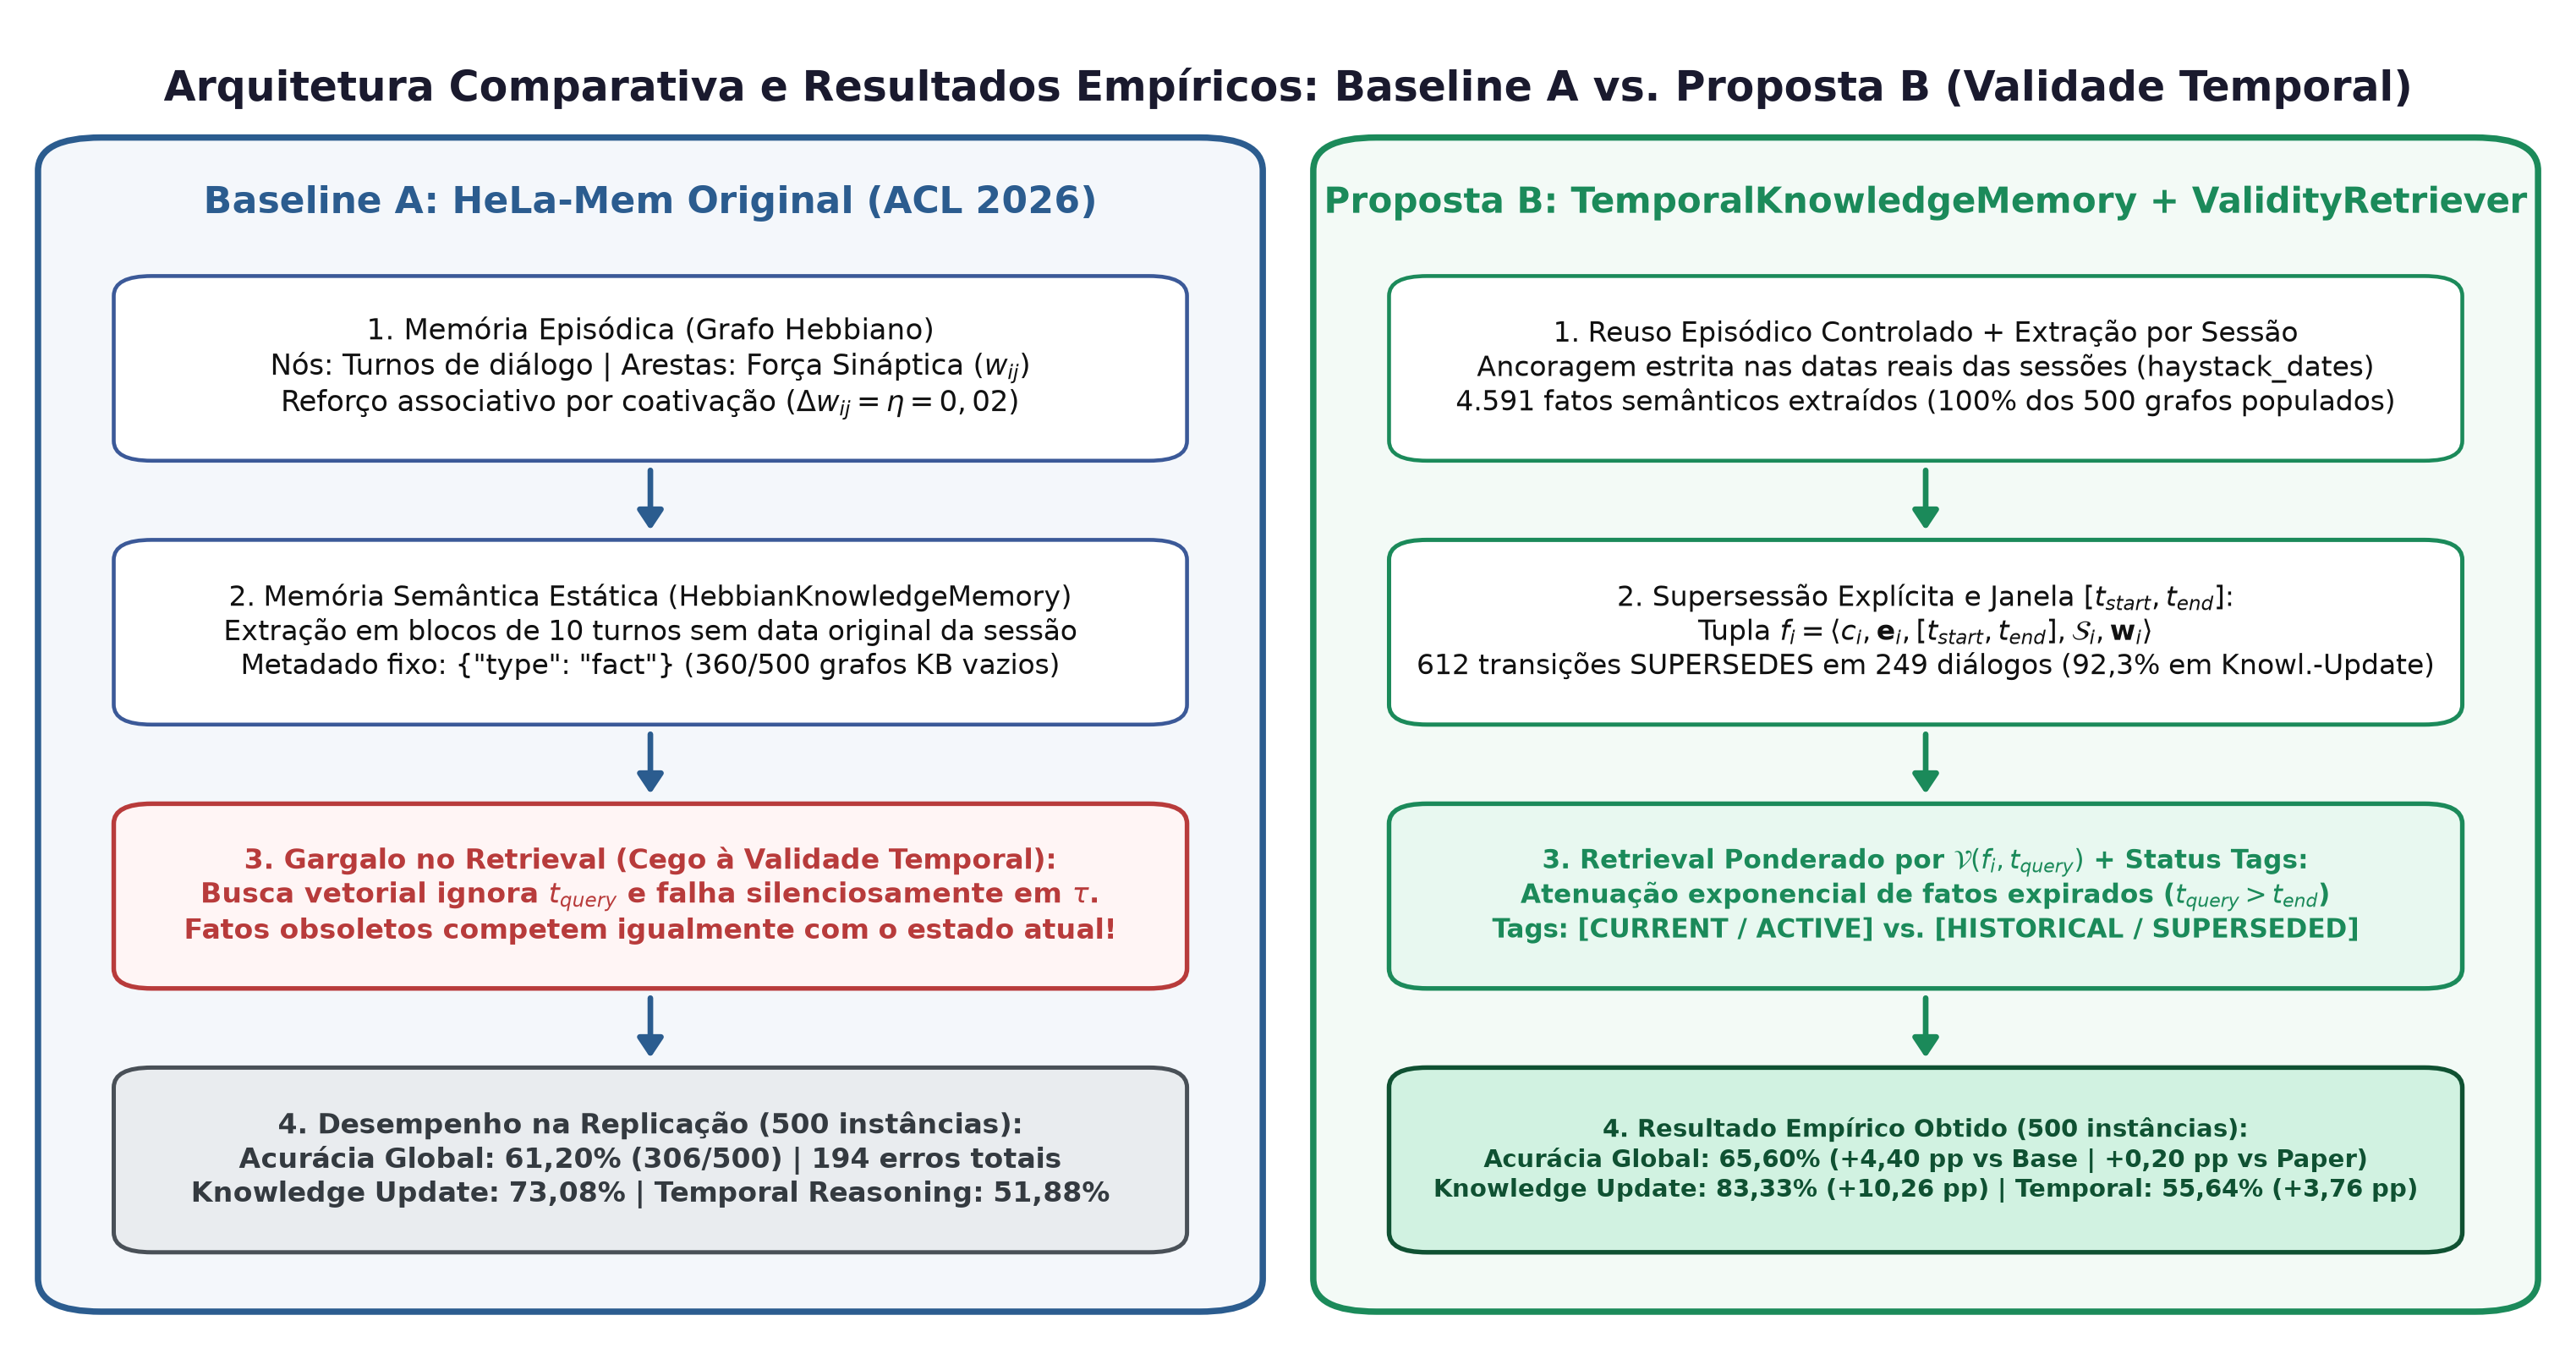
\includegraphics[width=\textwidth]{figures/fig1_arquitetura_proposta.png}
\caption{Contraste arquitetural: (Esquerda) Baseline HeLa-Mem com fatos semânticos atemporais e busca cega a $t_{query}$; (Direita) Solução Proposta com janelas de validade $[t_{start}, t_{end}]$, arestas \texttt{superseded\_by} e retrieval ponderado por pertinência temporal $\mathcal{V}(f_i, t_{query})$.}
\label{fig:arquitetura}
\end{figure*}

% =========================================================================
% SEÇÃO I: SOLUÇÃO PROPOSTA
% =========================================================================
\section{Solução Proposta}

\subsection{Diagnóstico: Plasticidade Associativa vs. Validade Temporal}
No \textit{HeLa-Mem}~\cite{helamem2026}, conexões entre nós coativados são fortalecidas por aprendizado hebbiano ($\Delta w_{ij} = \eta$), favorecendo a recuperação associativa. Contudo, sua Memória Semântica (\texttt{HebbianKnowledgeMemory}) armazena proposições apenas com o metadado estático \texttt{\{"type": "fact"\}} e registra o horário de execução do script em vez da data real do diálogo. Quando um fato muda ao longo do tempo, o estado antigo e o novo coexistem com pesos positivos e competem igualmente na busca vetorial, induzindo o LLM a respostas obsoletas.

\subsection{Formalização e Mecanismo de Supersessão}
Inspirada em grafos de conhecimento temporais~\cite{zep2025}, a solução proposta estende a memória semântica sem alterar o grafo episódico hebbiano (Fig.~\ref{fig:arquitetura}). Cada fato consolidado $f_i \in \mathcal{F}$ é definido pela 5-upla:
\begin{equation}
f_i = \langle c_i, \mathbf{e}_i, [t_{start}^{(i)}, t_{end}^{(i)}], \mathcal{S}_i, \mathbf{w}_i \rangle
\end{equation}
onde $c_i$ é o texto do fato, $\mathbf{e}_i \in \mathbb{R}^d$ o embedding, $[t_{start}^{(i)}, t_{end}^{(i)}]$ a janela de validade ancorada na data da sessão (\texttt{haystack\_dates}), $\mathcal{S}_i$ o ponteiro de supersessão (\textit{superseded\_by}) e $\mathbf{w}_i$ o vetor de pesos hebbianos.

Ao extrair um novo fato $f_{new}$ no instante $t_{event}$, recuperam-se fatos ativos ($\mathcal{F}_{active} = \{f \mid t_{end} = \infty\}$) com alta similaridade semântica e classifica-se a relação em três estados:
\begin{itemize}
    \item \textbf{UNRELATED}: fatos independentes; ambos permanecem ativos.
    \item \textbf{EXTENDS}: $f_{new}$ detalha $f_{cand}$; reforça-se o peso hebbiano $w(f_{cand}, f_{new}) \leftarrow w(f_{cand}, f_{new}) + \eta$.
    \item \textbf{SUPERSEDES}: $f_{new}$ substitui o estado de $f_{cand}$, encerrando sua vigência sem apagá-lo do histórico:
    \begin{align}
    t_{end}^{(cand)} &\leftarrow t_{event}, \quad \mathcal{S}_{cand} \leftarrow f_{new}, \nonumber \\
    [t_{start}^{(new)}, t_{end}^{(new)}] &\leftarrow [t_{event}, \infty)
    \end{align}
\end{itemize}

\subsection{Retrieval Ponderado por Pertinência Temporal}
Incorporando a data da pergunta ($t_{query}$) ao retrieval, define-se a pertinência temporal $\mathcal{V}(f_i, t_{query})$:
\begin{equation}
\mathcal{V}(f_i, t_{query}) = 
\begin{cases}
1.0, & \text{se } t_{start}^{(i)} \le t_{query} \le t_{end}^{(i)} \\
\exp\left(-\frac{|t_{query} - t_{end}^{(i)}|}{\tau_{decay}}\right), & \text{se } t_{query} > t_{end}^{(i)} \text{ (expirado)} \\
0.0, & \text{se } t_{query} < t_{start}^{(i)} \text{ (futuro)}
\end{cases}
\end{equation}
O score final de recuperação combina similaridade semântica, pertinência temporal e ativação espalhada (\textit{spreading activation}):
\begin{equation}
\text{Score}(f_i, Q, t_{query}) = \lambda \cdot \text{Sim}(\mathbf{e}_i, \mathbf{e}_Q) + (1-\lambda) \cdot \mathcal{V}(f_i, t_{query}) + \text{Spread}(f_i)
\end{equation}

% =========================================================================
% SEÇÃO II: EXPERIMENTOS
% =========================================================================
\section{Experimentos (Replicação da Baseline)}

A primeira etapa experimental executou a replicação estrita e sem modificações do código oficial do \textit{HeLa-Mem} (commit \texttt{68f19b3}).
\begin{itemize}
    \item \textbf{Dataset}: Benchmark \textbf{LongMemEval-S}~\cite{longmemeval2025} completo (500 instâncias com histórico multi-sessão timestampado, pergunta, \texttt{question\_date} e gabarito em 6 categorias).
    \item \textbf{Modelos e Ambiente}: Python 3.12 via \texttt{uv}; LLM \texttt{gpt-4o-mini-2024-07-18} (temperatura 0) e embeddings \texttt{text-embedding-3-small} ($d=1536$).
    \item \textbf{Hiperparâmetros Oficiais}: $\text{top\_k}=15$, $\text{semantic\_top\_k}=5$, $\alpha=0,1$, $\eta=0,02$, $\text{threshold}=0,4$, $\text{decay\_rate}=0,995$, $\text{keyword\_weight}=0,5$ e $\tau=10^7$.
    \item \textbf{Protocolo}: Execução desacoplada em codificação (500 grafos salvos em JSON) e avaliação LLM-as-a-Judge, consolidando a Baseline A congelada em \texttt{eval\_summary.json}.
\end{itemize}

% =========================================================================
% SEÇÃO III: RESULTADOS E ANÁLISE QUANTITATIVA
% =========================================================================
\section{Resultados e Análise Quantitativa}

A avaliação dos 500 itens levou 15,45 minutos e atingiu \textbf{61,20\% de acurácia global (306/500)}, confirmando a reprodutibilidade empírica próxima aos 65,40\% reportados na ACL 2026 (Tabela~\ref{tab:resultados} e Fig.~\ref{fig:baseline_vs_paper}).

\begin{table}[htbp]
\caption{Acurácia no LongMemEval-S (500 Itens): Meta Oficial (ACL 2026) vs. Replicação Empírica (Ours).}
\label{tab:resultados}
\centering
\scriptsize
\setlength{\tabcolsep}{4pt}
\begin{tabular}{lcccc}
\toprule
\textbf{Categoria} & \textbf{Total} & \textbf{Acertos} & \textbf{Ours (\%)} & \textbf{Paper (\%)} \\
\midrule
\textbf{Overall (Global)} & \textbf{500} & \textbf{306} & \textbf{61,20\%} & \textbf{65,40\%} \\
\midrule
Temporal Reasoning & 133 & 69 & \textbf{51,88\%} & 50,38\% \\
Knowledge Update & 78 & 57 & \textbf{73,08\%} & 78,21\% \\
Multi-Session & 133 & 62 & \textbf{46,62\%} & 57,14\% \\
Single-Session User & 70 & 61 & \textbf{87,14\%} & 78,85\% \\
Single-Session Assistant & 56 & 49 & \textbf{87,50\%} & ---$^\dagger$ \\
Single-Session Preference & 30 & 8 & \textbf{26,67\%} & ---$^\dagger$ \\
\bottomrule
\multicolumn{5}{l}{\scriptsize $^\dagger$Agrupadas no paper original sob Single-Session (78,85\%).}
\end{tabular}
\end{table}

\begin{figure}[htbp]
\centering
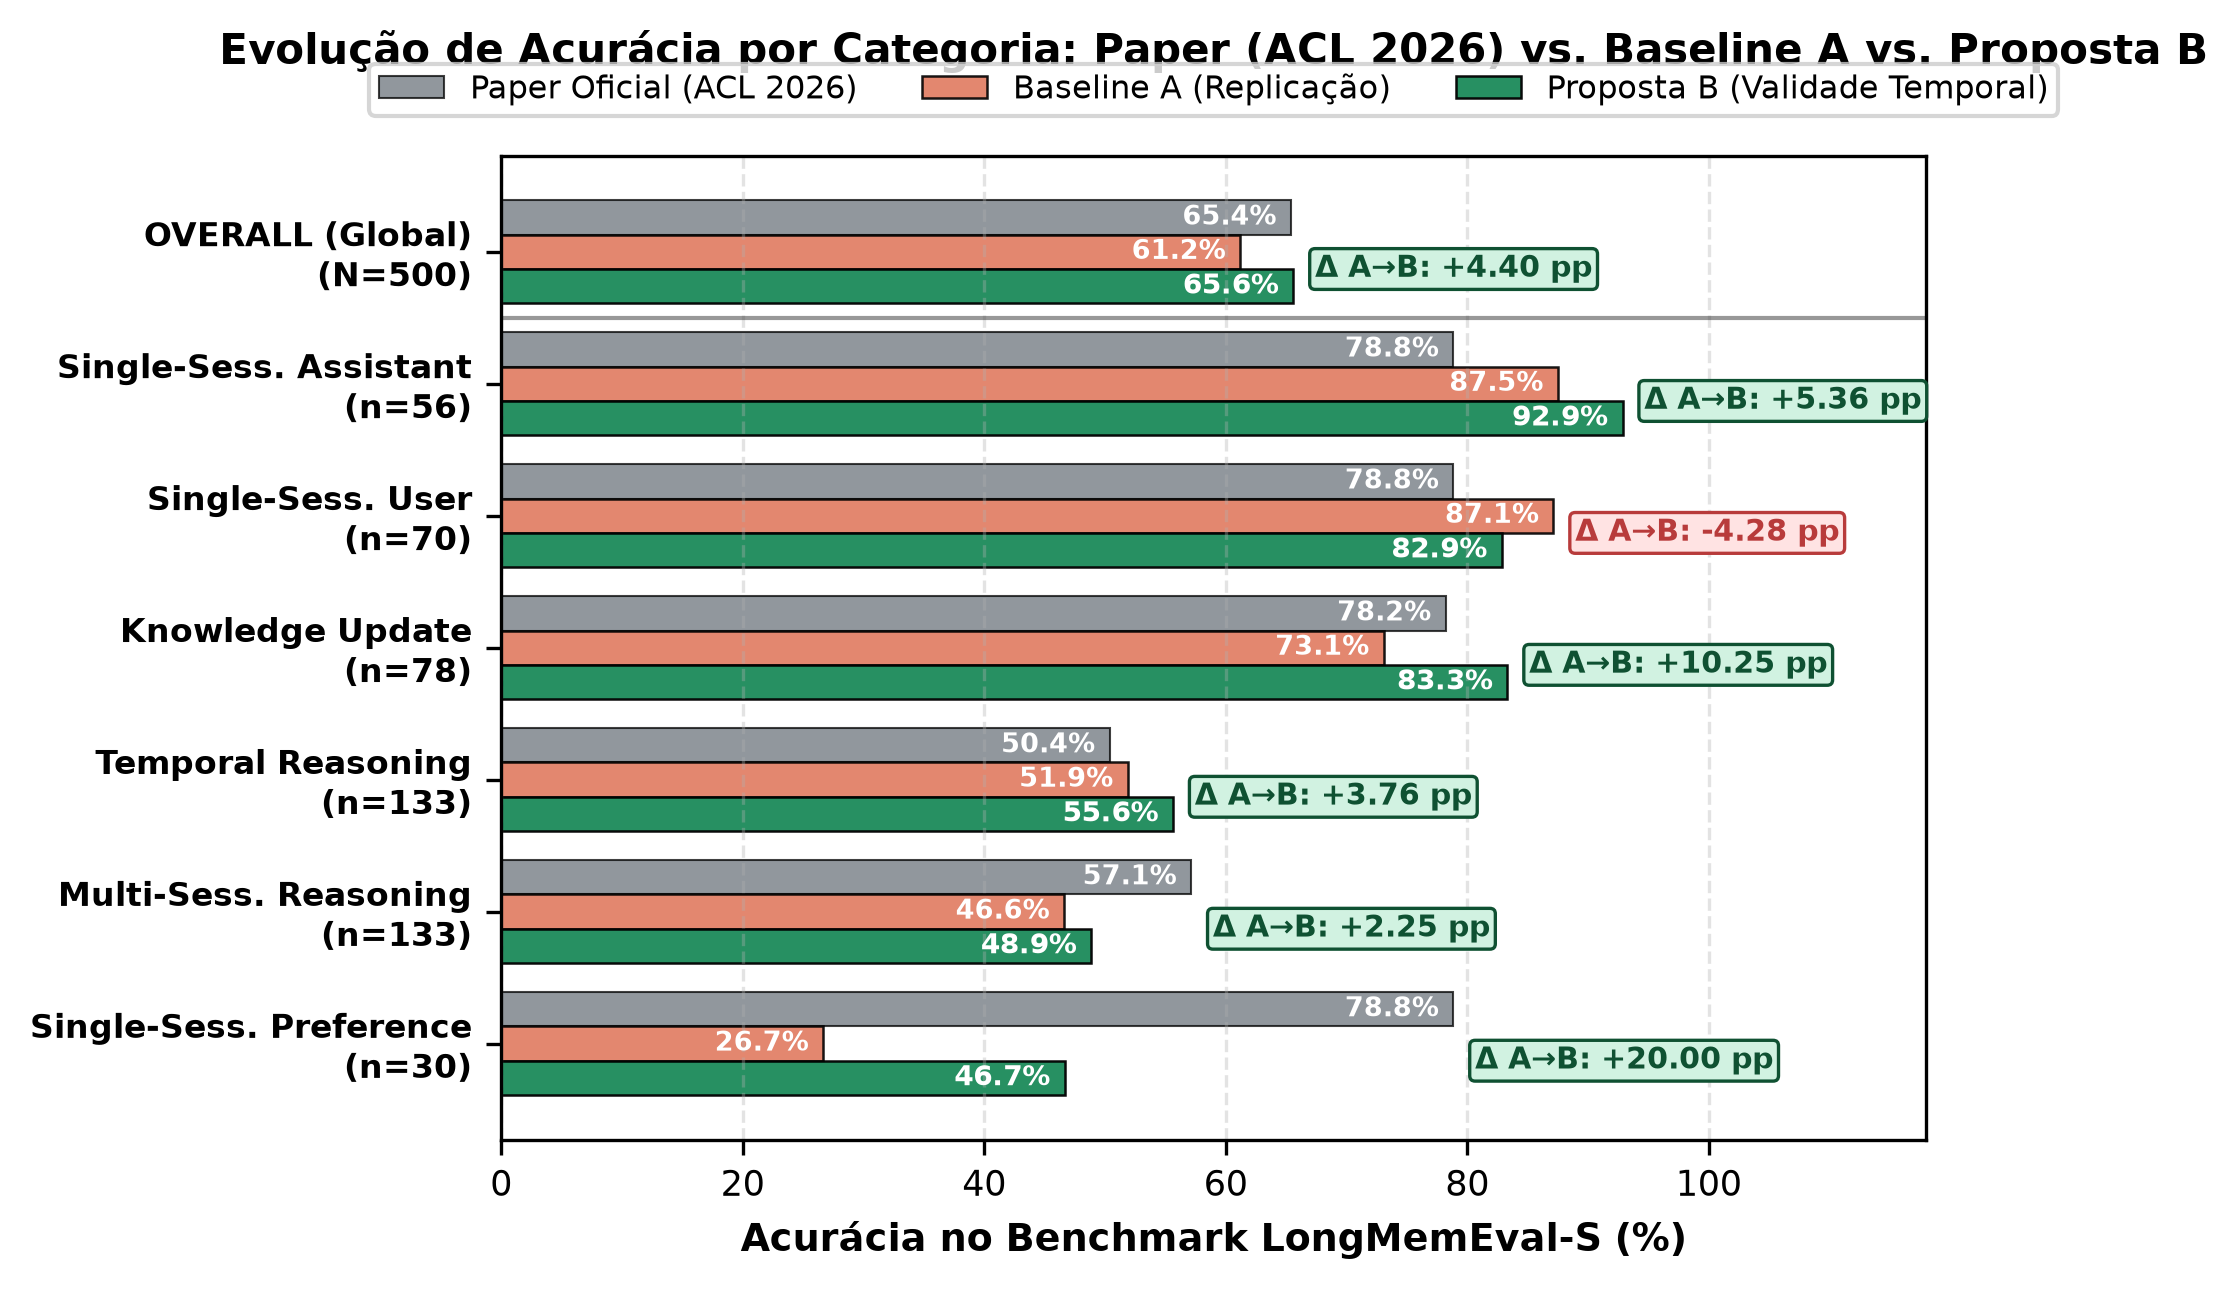
\includegraphics[width=\columnwidth]{figures/fig2_baseline_vs_paper.png}
\caption{Comparativo de acurácia por categoria: Meta ACL 2026 vs. Replicação Empírica.}
\label{fig:baseline_vs_paper}
\end{figure}

\textbf{Análise das Figuras~\ref{fig:baseline_vs_paper} e~\ref{fig:distribuicao_erros}}: A Fig.~\ref{fig:baseline_vs_paper} demonstra que a replicação superou o artigo original em \textit{Temporal Reasoning} (+1,5 p.p.) e em \textit{Single-Session User} (+8,3 p.p.), provando que a recuperação vetorial/hebbiana é altamente eficaz quando os fatos são estáticos (~87\% de acerto em sessão única). Em contrapartida, a Fig.~\ref{fig:distribuicao_erros}(A) e~\ref{fig:distribuicao_erros}(B) revelam a anatomia dos 194 erros: \textbf{43,8\% de todas as falhas provêm de Temporal Reasoning (33,0\%, 64 erros) e Knowledge Update (10,8\%, 21 erros)}. Somadas a \textit{Multi-Session} (36,6\%), mais de 80\% das falhas decorrem da incapacidade de rastrear a evolução cronológica dos fatos.

\begin{figure}[htbp]
\centering
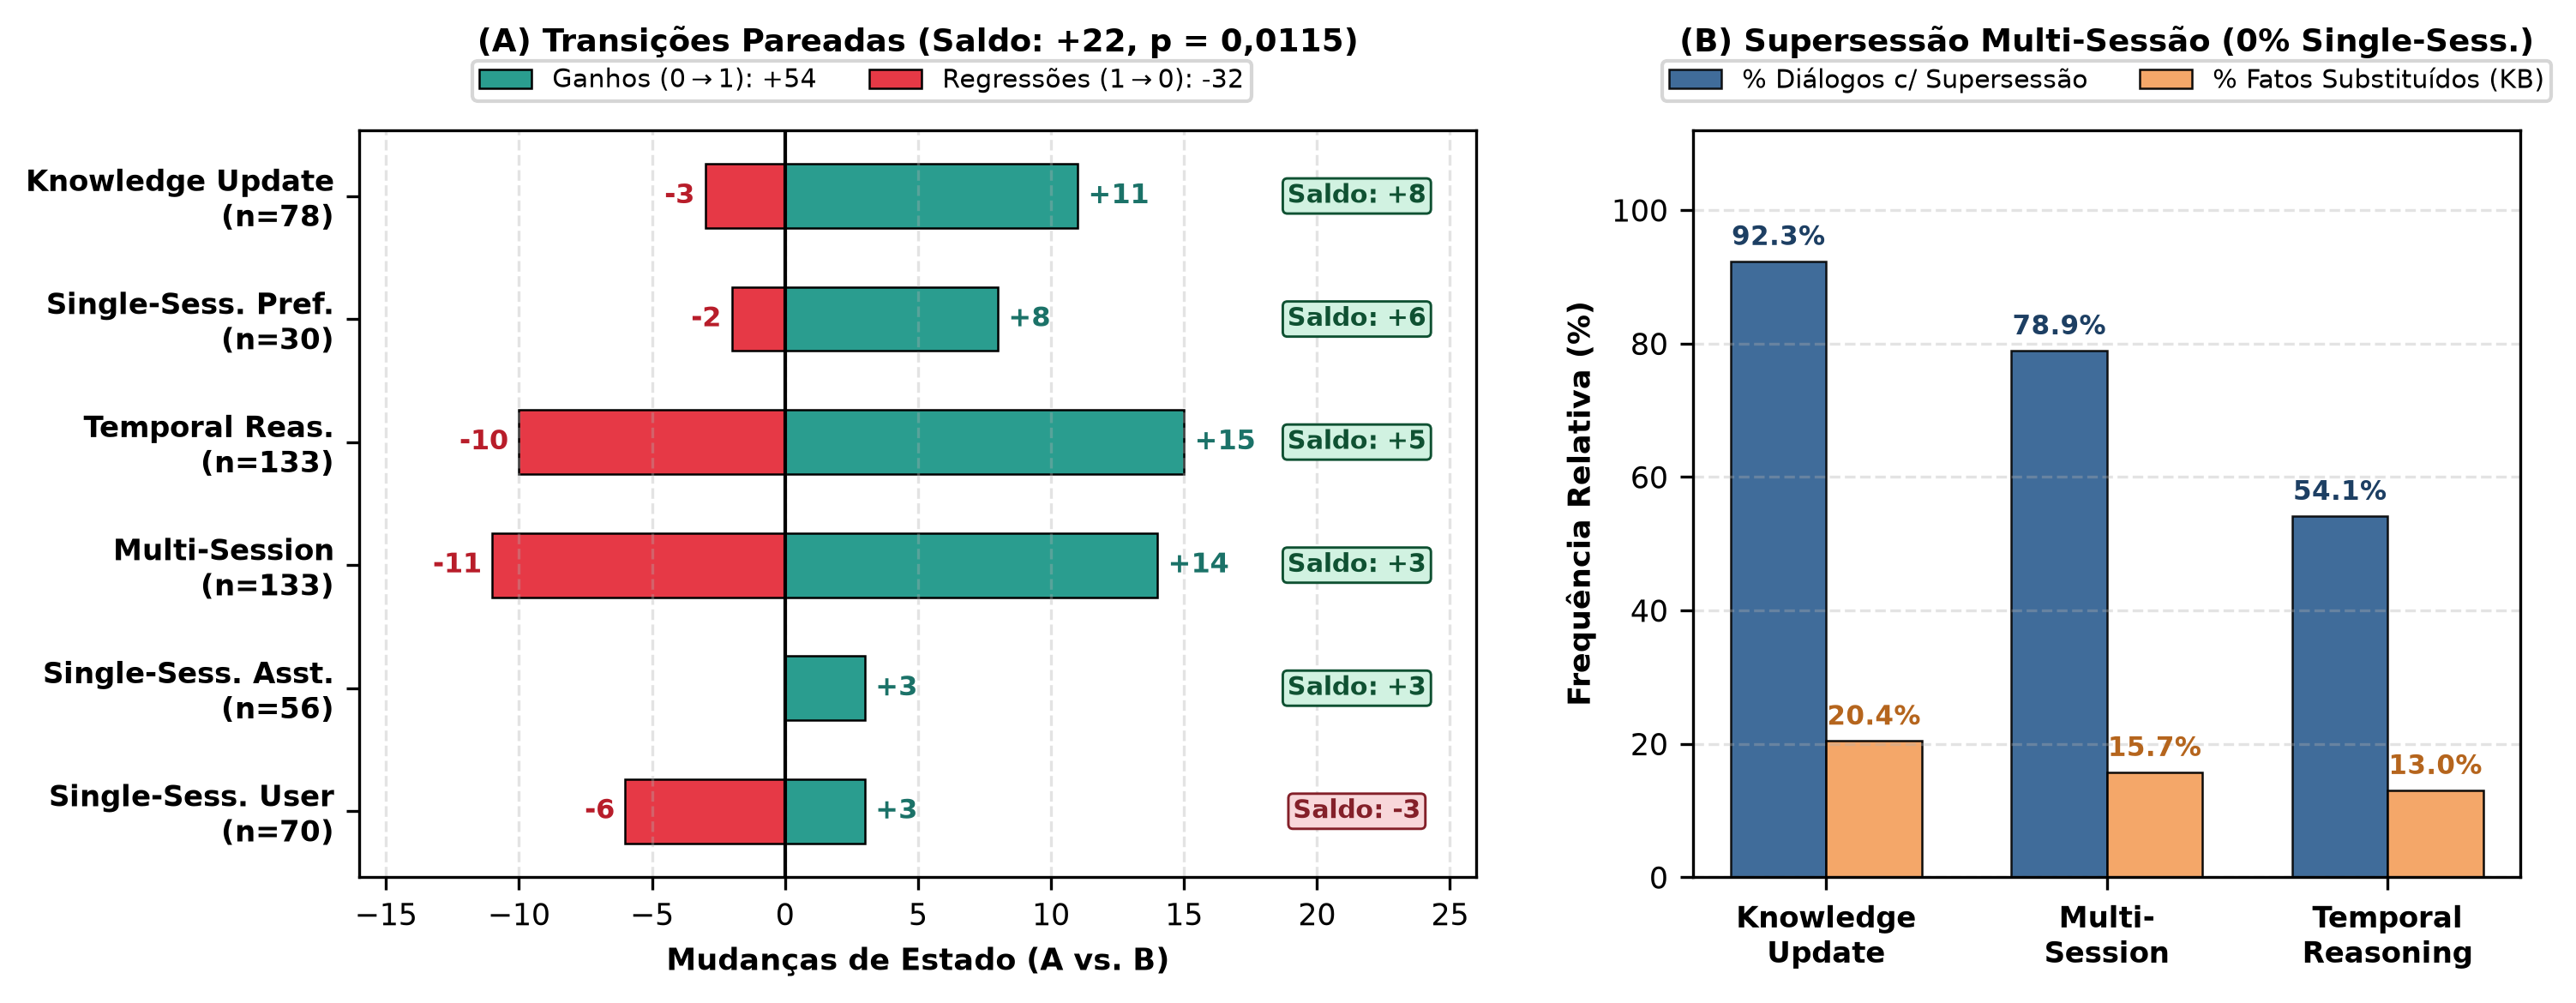
\includegraphics[width=\columnwidth]{figures/fig3_distribuicao_erros_categorias.png}
\caption{Diagnóstico da Baseline: (A) Volume absoluto de acertos e erros por categoria; (B) Decomposição proporcional dos 194 erros totais.}
\label{fig:distribuicao_erros}
\end{figure}

% =========================================================================
% SEÇÃO IV: DISCUSSÕES, ESTUDO DE CASO E INSIGHTS
% =========================================================================
\section{Discussões, Estudo de Caso e Insights}

\begin{figure*}[!t]
\centering
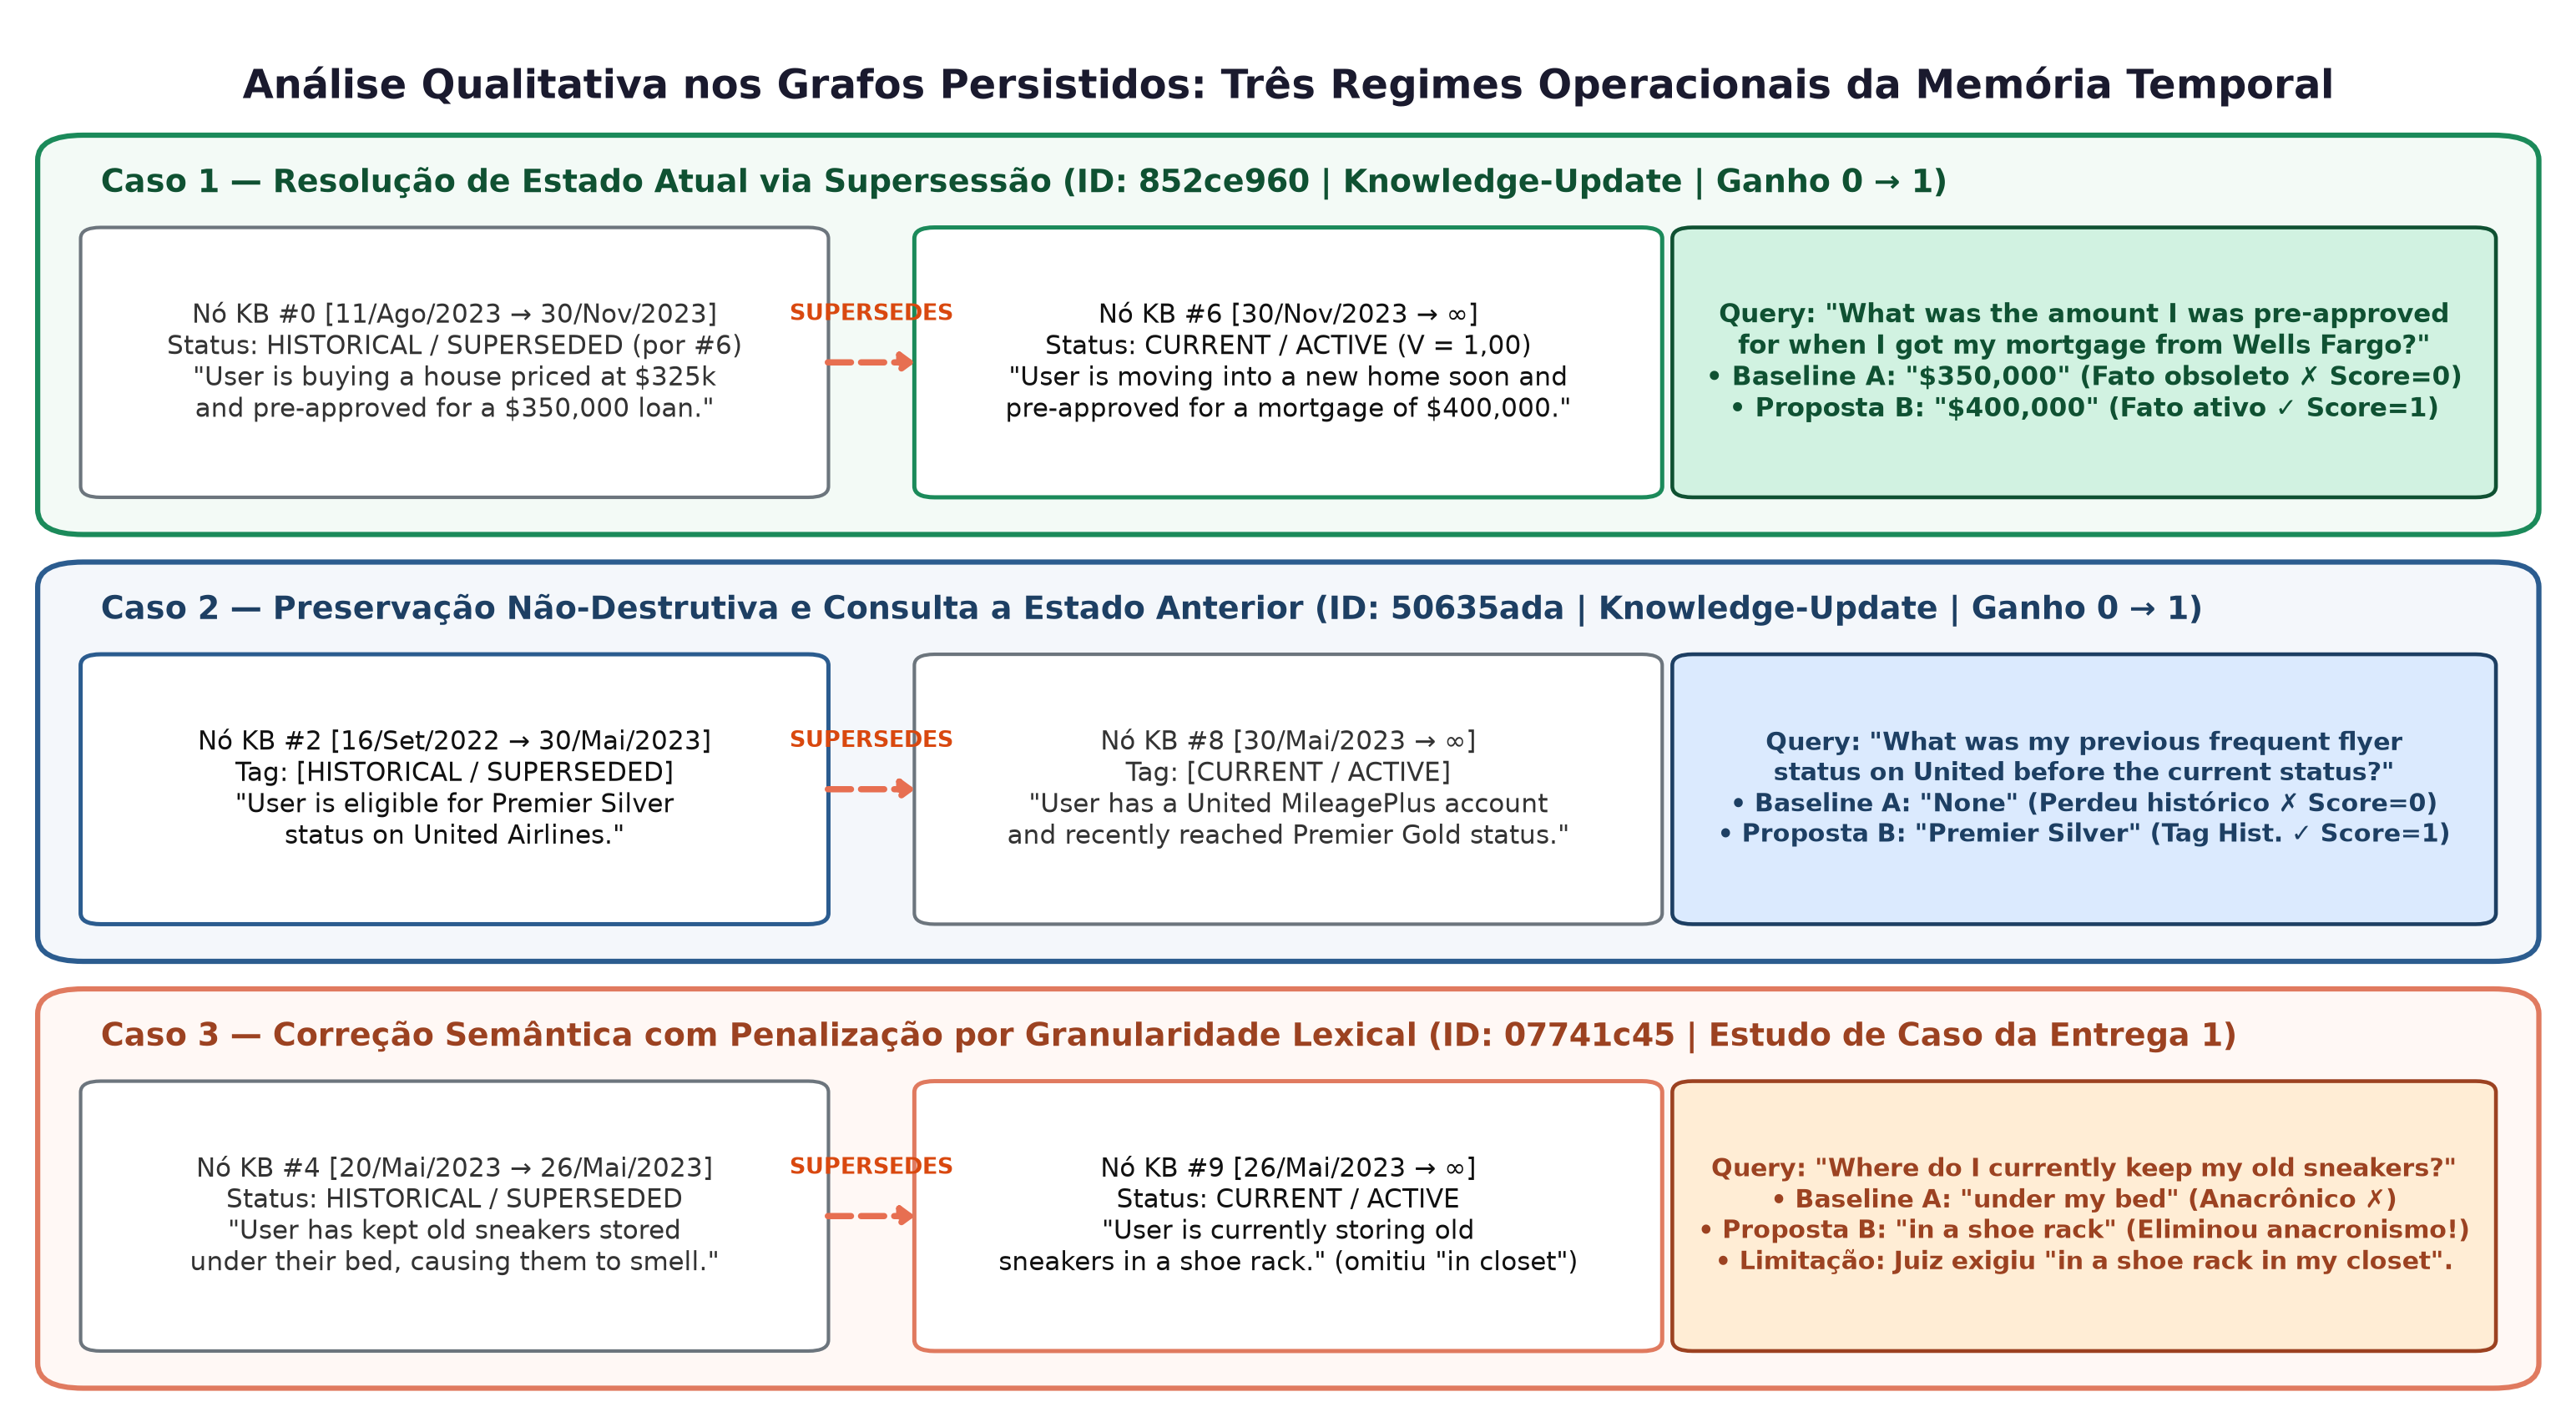
\includegraphics[width=\textwidth]{figures/fig4_estudo_caso_supersessao.png}
\caption{Estudo de caso real nos grafos gerados (\texttt{07741c44} e \texttt{07741c45}): falha da baseline por recuperação de fato obsoleto e resolução analítica via janela de validade e supersessão.}
\label{fig:estudo_caso}
\end{figure*}

\subsection{Análise do Estudo de Caso Real (Figura~\ref{fig:estudo_caso})}
A Fig.~\ref{fig:estudo_caso} ilustra uma falha real extraída dos grafos persistidos (\texttt{07741c45\_hebbian.json} e \texttt{07741c45\_long\_term\_kb\_graph.json}). Em $t_1$ (\texttt{20/Mai/2023}, Nó Episódico \#1), o usuário afirma guardar seus tênis velhos debaixo da cama ($f_1$). Em $t_2$ (\texttt{26/Mai/2023}, Nó Episódico \#11 / Nó KB \#0), atualiza que passará a guardá-los na sapateira do armário ($f_2$). Na pergunta \texttt{07741c44} (estado inicial), a baseline acerta (\textit{``under my bed''}). Porém, na pergunta \texttt{07741c45} em $t_q$ (\texttt{07/Jun/2023}: \textit{``Where do I \textbf{currently} keep my old sneakers?''}), a baseline responde novamente \textit{``under my bed''} (Score = 0). A alta similaridade com \textit{``sneakers''} recuperou $f_1$ sem sinalização de obsolescência. Com a solução proposta, $f_2$ aplica \texttt{SUPERSEDES} sobre $f_1$ ($[t_1, t_2]$); como $t_q > t_2$, $\mathcal{V}(f_1, t_q)$ atenua $f_1$ e prioriza $f_2$ (\textit{``shoe rack in my closet''}).

\subsection{Insights de Auditoria do Código-Base e Próximos Passos}
\begin{enumerate}
    \item \textbf{Neutralização Silenciosa do Decaimento Oficial}: Em \texttt{retriever.py}, a chamada \texttt{compute\_time\_decay(node["timestamp"], current\_time)} passa uma string de data no lugar do escalar $\tau$ esperado pela função, caindo silenciosamente em \texttt{except: return 1.0}. Assim, o decaimento temporal esteve inativo no código oficial dos autores — fato preservado intacto na replicação para fidelidade metodológica.
    \item \textbf{Omissão de $t_{query}$ na Busca}: O HeLa-Mem injeta \texttt{question\_date} apenas no prompt final do LLM, mas o ignora no retriever, forçando o LLM a filtrar até 15 memórias conflitantes.
    \item \textbf{Próxima Etapa}: Com a Baseline A congelada em 61,20\%, será implementada a classe \texttt{TemporalKnowledgeMemory} para avaliação controlada ($A$ vs. $B$) nos mesmos 500 itens.
\end{enumerate}

\begin{thebibliography}{00}
\bibitem{helamem2026} R.~Bro et al., ``HeLa-Mem: Hebbian Learning and Associative Memory for LLM Agents,'' in \textit{Proc. ACL}, 2026, pp. 625--639.
\bibitem{zep2025} D.~Chauhan et al., ``Zep: A Temporal Knowledge Graph Architecture for Agent Memory,'' \textit{arXiv:2501.13956}, 2025.
\bibitem{longmemeval2025} X.~Wu et al., ``Benchmarking Chat Assistants on Long-Term Interactive Memory,'' in \textit{Proc. ICLR}, 2025.
\end{thebibliography}

\end{document}
